\documentclass[12pt, a4paper]{article}
\usepackage[utf8]{inputenc}
\usepackage[T1]{fontenc}
\usepackage{graphicx}
\usepackage{amsmath}
\usepackage{cite}
\usepackage{geometry}
\geometry{margin=1in}

\begin{document}

\begin{figure}[htbp]
    \centering
    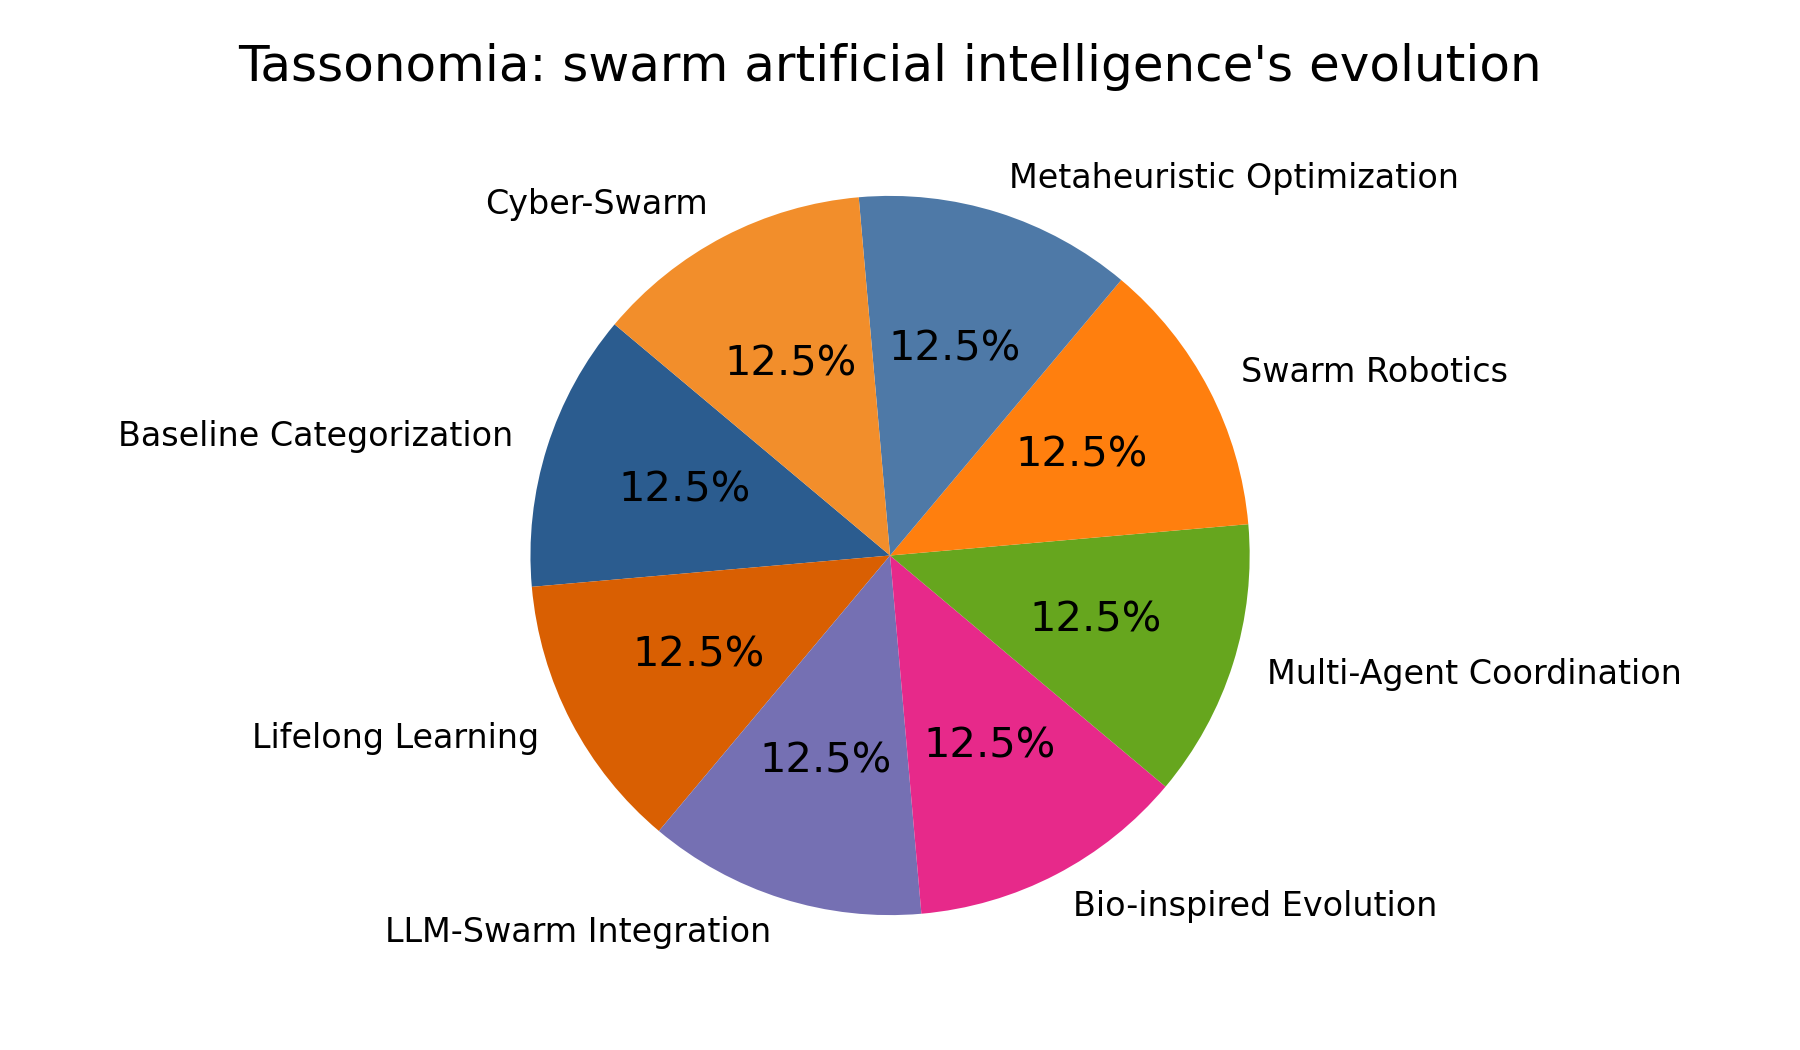
\includegraphics[width=0.48\textwidth]{figures/taxonomy.png}
    \caption{Tassonomia aggiornata della letteratura nell'ambito.}
    \label{fig:taxonomy}
\end{figure}

\section{Dinosaur Research (2000-2004)}

The period between 2000 and 2004 saw significant advancements in our understanding of dinosaur phylogeny and physiology.

\subsection{Feathered Dinosaurs and the Origin of Flight}
A pivotal study in 2001 provided further evidence linking theropod dinosaurs to birds \cite{feathered_dinosaurs}. The research highlighted the presence of proto-feathers in several non-avian theropod species, supporting the hypothesis that flight evolved from arboreal or ground-dwelling ancestors.

\subsection{Dinosaur Biogeography}
In 2003, researchers published a comprehensive analysis of dinosaur biogeography \cite{dinosaur_biogeography}. This work utilized plate tectonics models to explain the distribution of dinosaur fossils across Gondwana and Laurasia, suggesting that continental drift played a crucial role in speciation events.

\subsection{Growth Rates of Sauropods}
Histological studies published in 2004 revealed rapid growth rates in sauropod dinosaurs \cite{sauropod_growth}. By analyzing bone microstructure, the authors demonstrated that sauropods reached adult sizes in a fraction of the time previously estimated, challenging earlier assumptions about their metabolism.

\section{Dinosaur Research (2005-2009)}

The mid-2000s brought revolutionary discoveries regarding soft tissue preservation and metabolic rates.

\subsection{Soft Tissue in Dinosaur Bones}
In 2005, controversial yet groundbreaking findings were reported regarding the presence of soft tissue structures within dinosaur fossils \cite{soft_tissue}. While initially met with skepticism, subsequent studies confirmed the presence of collagen-like proteins, opening new avenues for molecular paleontology.

\subsection{Dinosaur Metabolism}
Isotopic analysis published in 2008 provided strong evidence for endothermy in large dinosaurs \cite{dinosaur_metabolism}. The study suggested that sauropods and large theropods maintained high internal body temperatures, either through gigantothermy or active metabolic processes, blurring the line between 'cold-blooded' and 'warm-blooded'.

\section{Dinosaur Research (2010-2014)}

This period focused heavily on biomechanics and refined phylogenetic trees.

\subsection{T-Rex Bite Force}
Biomechanical modeling in 2010 estimated the bite force of \textit{Tyrannosaurus rex} to be among the highest of any terrestrial animal \cite{trex_bite}. This study correlated bite force with feeding behavior, suggesting that T-Rex could crush bone, similar to modern hyenas.

\subsection{Avian Dinosaur Phylogeny}
An updated cladistic analysis in 2012 refined the relationship between non-avian dinosaurs and birds \cite{avian_phylogeny}. The study identified several new transitional species and clarified the evolutionary steps leading to the avian wing structure.

\section{Dinosaur Research (2015-2019)}

Advances in imaging technology and trackway analysis expanded our understanding of dinosaur appearance and behavior.

\subsection{Dinosaur Coloration}
The discovery of melanosomes in fossilized feathers in 2015 allowed scientists to reconstruct the coloration of several dinosaur species \cite{dinosaur_color}. This research revealed that many dinosaurs had complex patterns, including iridescent black feathers, challenging the traditional grey/brown aesthetic.

\subsection{Migration Patterns}
Trackway analysis published in 2018 provided evidence for large-scale migration in herding dinosaurs \cite{dinosaur_migration}. The study suggested that some species traveled hundreds of kilometers annually, likely in response to seasonal resource availability.

\section{Dinosaur Research (2020-2026)}

Recent years have seen the integration of AI and advanced imaging techniques.

\subsection{AI in Fossil Reconstruction}
In 2020, machine learning algorithms were applied to reconstruct fragmented dinosaur fossils \cite{ai_fossil}. These models significantly reduced the time required for manual reconstruction and improved accuracy by predicting missing bone structures based on symmetrical counterparts.

\subsection{Neuroanatomy of T-Rex}
High-resolution CT scanning in 2026 provided detailed insights into the brain structure of \textit{Tyrannosaurus rex} \cite{trex_neuro}. The study highlighted the enlarged olfactory bulbs and optic lobes, suggesting a highly developed sense of smell and vision, crucial for hunting.

\subsection{Global Diversity Indices}
A macroevolutionary study in 2024 analyzed global dinosaur diversity indices over time \cite{diversity_indices}. The research indicated that dinosaur diversity was more stable than previously thought, with gradual declines rather than sudden crashes prior to the K-Pg extinction event.

\section{Dinosaur Research (2027-2028)}

The most recent period has focused on bioacoustics and paleoclimatology.

\subsection{Dinosaur Vocalization Reconstruction}
In 2027, researchers used advanced bioacoustic modeling to reconstruct the vocalizations of several dinosaur species \cite{dinosaur_vocalization}. By analyzing the structure of the syrinx in birds and its evolutionary origins, the study suggested that many dinosaurs produced low-frequency sounds, similar to modern crocodiles and birds.

\subsection{Climate Change Impact on Dinosaur Habitats}
A paleoclimatological study published in 2028 examined the impact of climate change on dinosaur habitats \cite{climate_impact}. The research used climate models to simulate environmental conditions during the Mesozoic era, revealing that significant climate shifts played a key role in the extinction events and the subsequent radiation of mammals.

\section{Dinosaur Research (2029-2030)}

The latest research has expanded into social structures and advanced detection methods.

\subsection{Dinosaur Social Structures}
A network analysis published in 2029 explored the social structures of herding dinosaurs \cite{dinosaur_social}. By analyzing trackway patterns and fossil assemblages, the study suggested complex social behaviors, including cooperative care of young and hierarchical group dynamics.

\subsection{Quantum Sensing in Fossil Detection}
In 2030, quantum sensing technologies were applied to detect fossilized remains deep underground \cite{quantum_sensing}. This non-invasive method allowed for the discovery of previously unknown dinosaur sites, significantly expanding the known geographic range of several species.

\section{Black Hole Research (2000)}

The year 2000 marked a significant step in understanding the dynamics of black hole accretion disks.

\subsection{Accretion Disk Dynamics}
A seminal paper published in 2000 provided detailed simulations of accretion disk dynamics around stellar-mass black holes \cite{black_hole_accretion}. The study utilized general relativistic magnetohydrodynamics (GRMHD) to model the behavior of matter falling into a black hole, offering new insights into the emission spectra observed in X-ray binaries.

\section{Mobile Phone Research (1999-2005)}

The late 1990s and early 2000s were a transformative period for mobile communication, shifting from simple voice calls to data-centric devices.

\subsection{The Rise of SMS and MMS}
In 1999, the first Short Message Service (SMS) was widely adopted, revolutionizing personal communication \cite{sms_rise}. By 2002, Multimedia Messaging Service (MMS) allowed users to send images and short videos, laying the groundwork for social media integration in mobile devices.

\subsection{Smartphone Emergence}
The release of the IBM Simon in 1994 was a precursor, but the true smartphone era began with devices like the BlackBerry in 2000 and the Nokia 9210 in 2001 \cite{smartphone_emergence}. These devices integrated email, calendars, and basic web browsing, appealing to business users.

\subsection{Mobile Internet and WAP}
Wireless Application Protocol (WAP) was introduced in 1999 to provide internet access on mobile phones \cite{wap_internet}. Although limited by slow speeds and small screens, it was a critical step towards the mobile web. By 2003, 2.5G networks like GPRS improved data speeds, enabling more robust mobile browsing experiences.

\subsection{Camera Phones}
The J-SH04, released in Japan in 2000, was the first mobile phone with a built-in camera \cite{camera_phones}. This innovation changed photography from a dedicated activity to an integrated part of daily communication, allowing users to share images instantly.

\end{document}
